\documentclass{beamer}
\usepackage{amsmath}
\usepackage[utf8]{inputenc}
\usepackage{graphics}
\usepackage{hyperref}
\usepackage{xcolor}
\usepackage{wasysym}
\usepackage{listings}
\usepackage{tikz}
\usepackage{amssymb}
\usepackage[normalem]{ulem}
\usepackage{textcomp}
\usepackage{verbatim}
\usepackage[T1]{fontenc}
\usepackage{lmodern}
\usetikzlibrary{shapes.callouts,shadows, calc}

\tikzset{note/.style={rectangle callout, rounded corners,fill=gray!20,drop shadow,font=\footnotesize}}    
\newcommand{\tikzmark}[1]{\tikz[overlay,remember picture] \node (#1) {};}    

\newcounter{image}
\setcounter{image}{1}

\makeatletter
\newenvironment{btHighlight}[1][]
{\begingroup\tikzset{bt@Highlight@par/.style={#1}}\begin{lrbox}{\@tempboxa}}
{\end{lrbox}\bt@HL@box[bt@Highlight@par]{\@tempboxa}\endgroup}

\newcommand\btHL[1][]{%
  \begin{btHighlight}[#1]\bgroup\aftergroup\bt@HL@endenv%
}
\def\bt@HL@endenv{%
  \end{btHighlight}%   
  \egroup
}
\newcommand{\bt@HL@box}[2][]{%
  \tikz[#1]{%
    \pgfpathrectangle{\pgfpoint{0pt}{0pt}}{\pgfpoint{\wd #2}{\ht #2}}%
    \pgfusepath{use as bounding box}%
    \node[anchor=base west,rounded corners, fill=green!30,outer sep=0pt,inner xsep=0.2em, inner ysep=0.1em,  #1](a\theimage){\usebox{#2}};
  }%
 \stepcounter{image}
}
\makeatother

\usetheme{Warsaw}
\usecolortheme{lily}
\setbeamercovered{transparent}
\setbeamertemplate{headline}{
  \begin{beamercolorbox}{section in head/foot}
    \vskip2pt\insertnavigation{\paperwidth}\vskip2pt
  \end{beamercolorbox}
}

\setbeamertemplate{footline}{
}

\author{
  {\tiny Tony Morris\\}
}

\xdefinecolor{darkgreen}{rgb}{0,0.35,0}
\lstset{
  tabsize=2,
  basicstyle=\ttfamily,
  moredelim=**[is][\btHL]{`}{`}
}
\lstdefinestyle{java}{
  language=java,
  basicstyle=\footnotesize\ttfamily,
  stringstyle=\color{darkgreen}\ttfamily,
  commentstyle=\color{gray}\ttfamily,
  keywordstyle=\footnotesize\color{blue}\ttfamily,
  tabsize=2,
  moredelim=**[is][\btHL]{`}{`}
}
\lstdefinelanguage{scala}{
  morekeywords={abstract,case,catch,class,def,%
    do,else,extends,false,final,finally,%
    for,forSome,if,implicit,import,lazy,match,%
    new,null,object,override,package,%
    private,protected,requires,return,sealed,%
    super,this,throw,trait,true,try,%
    type,val,var,while,with,yield},
  otherkeywords={=,=>,<-,<\%,<:,>:,\#,@},
  sensitive=true,
  morecomment=[l]{//},
  morecomment=[n]{/*}{*/},
  morestring=[b]",
  morestring=[b]',
  morestring=[b]"""
}
\lstdefinelanguage{haskell}{
  morekeywords={class,instance,where,do,data,newtype,default,deriving,module},
  otherkeywords={<-},
  sensitive=true,
  morecomment=[l]{--},
  morecomment=[n]{\{-}{-\}}, 
  morestring=[b]",
  morestring=[b]',
  morestring=[b]"""
}
\lstdefinestyle{scala}{
  language=scala,
  basicstyle=\footnotesize\ttfamily,
  stringstyle=\color{darkgreen}\ttfamily,
  commentstyle=\color{gray}\ttfamily,
  keywordstyle=\footnotesize\color{blue}\ttfamily,
  tabsize=2,
  moredelim=**[is][\btHL]{`}{`}
}
\lstdefinestyle{haskell}{
  language=haskell,
  basicstyle=\tiny\ttfamily,
  stringstyle=\color{darkgreen}\ttfamily,
  commentstyle=\color{gray}\ttfamily,
  keywordstyle=\tiny\color{blue}\ttfamily,
  tabsize=2
}
% #866eaa
\definecolor{nicta-purple}{rgb}{0.5234,0.4297,0.6640}

\defbeamertemplate*{title page}{customized}[1][] {
  \centering
  \color{nicta-purple}
  \usebeamerfont{title}\inserttitle\par
  \bigskip
  \usebeamerfont{subtitle}\insertsubtitle\par
  \bigskip
  \bigskip
  \bigskip
  \bigskip
  \usebeamerfont{institute}\insertinstitute\par
  \bigskip
  \usebeamerfont{author}\insertauthor\par
  % \usebeamerfont{date}\insertdate\par
  \usebeamercolor[fg]{titlegraphic}\inserttitlegraphic
}

\logo{\includegraphics[height=0.8cm]{image/nicta.jpg}}

\begin{document}
\title{\large Parametricity}
\subtitle{\small Types Are Documentation}
\institute[NICTA]{}
\tiny{\date

}
\normalsize

\setbeamercovered{transparent}
\begin{frame}
  \titlepage
\end{frame}

\input{journey}
\begin{frame}
\frametitle{Scala}
\begin{itemize}
  \item We will use the Scala programming language for code examples
  \item However, the point of this talk does not relate to Scala specifically
\end{itemize}
\end{frame}

\begin{frame}
\frametitle{Scala}
\begin{center}
Other languages and syntax may be used to denote important concepts and ensure clarity
\end{center}
\begin{center}
\includegraphics[height=1.8cm]{image/tissues.jpg}
\end{center}
\end{frame}

\begin{frame}
\frametitle{Why Scala?}
\begin{itemize}
  \item Scala is a legacy hack used primarily by Damo for ciggy-butt brain
        programming
  \item Yet it is capable of achieving a high degree of code reasoning
  \item Speak up if unfamiliarity of syntax inhibits understanding
\end{itemize}
\end{frame}


\begin{frame}[fragile]
\frametitle{Lossful Reasoning}
\framesubtitle{Sacrificing efficiency to gain unreliability}
Suppose we encountered the following function definition:
\begin{lstlisting}[style=scala]
def add10(n: Int): Int
\end{lstlisting}
By the type alone, there are {$({2^{32}})^{2^{32}}$} possible implementations
\end{frame}

\begin{frame}[fragile]
\frametitle{Lossful Reasoning}
\framesubtitle{Sacrificing efficiency to gain unreliability}
We might form a suspicion that \lstinline[style=scala]$add10$ adds ten to its argument
\begin{lstlisting}[style=scala]
def `add10`(n: Int): Int
\end{lstlisting}
\begin{tikzpicture}[remember picture,overlay]
\coordinate (aa) at ($(a1)+(7,2.0)$);
\node[note,draw,callout relative pointer={($(aa)-(11.2,-3.7)$)},right] at (aa) {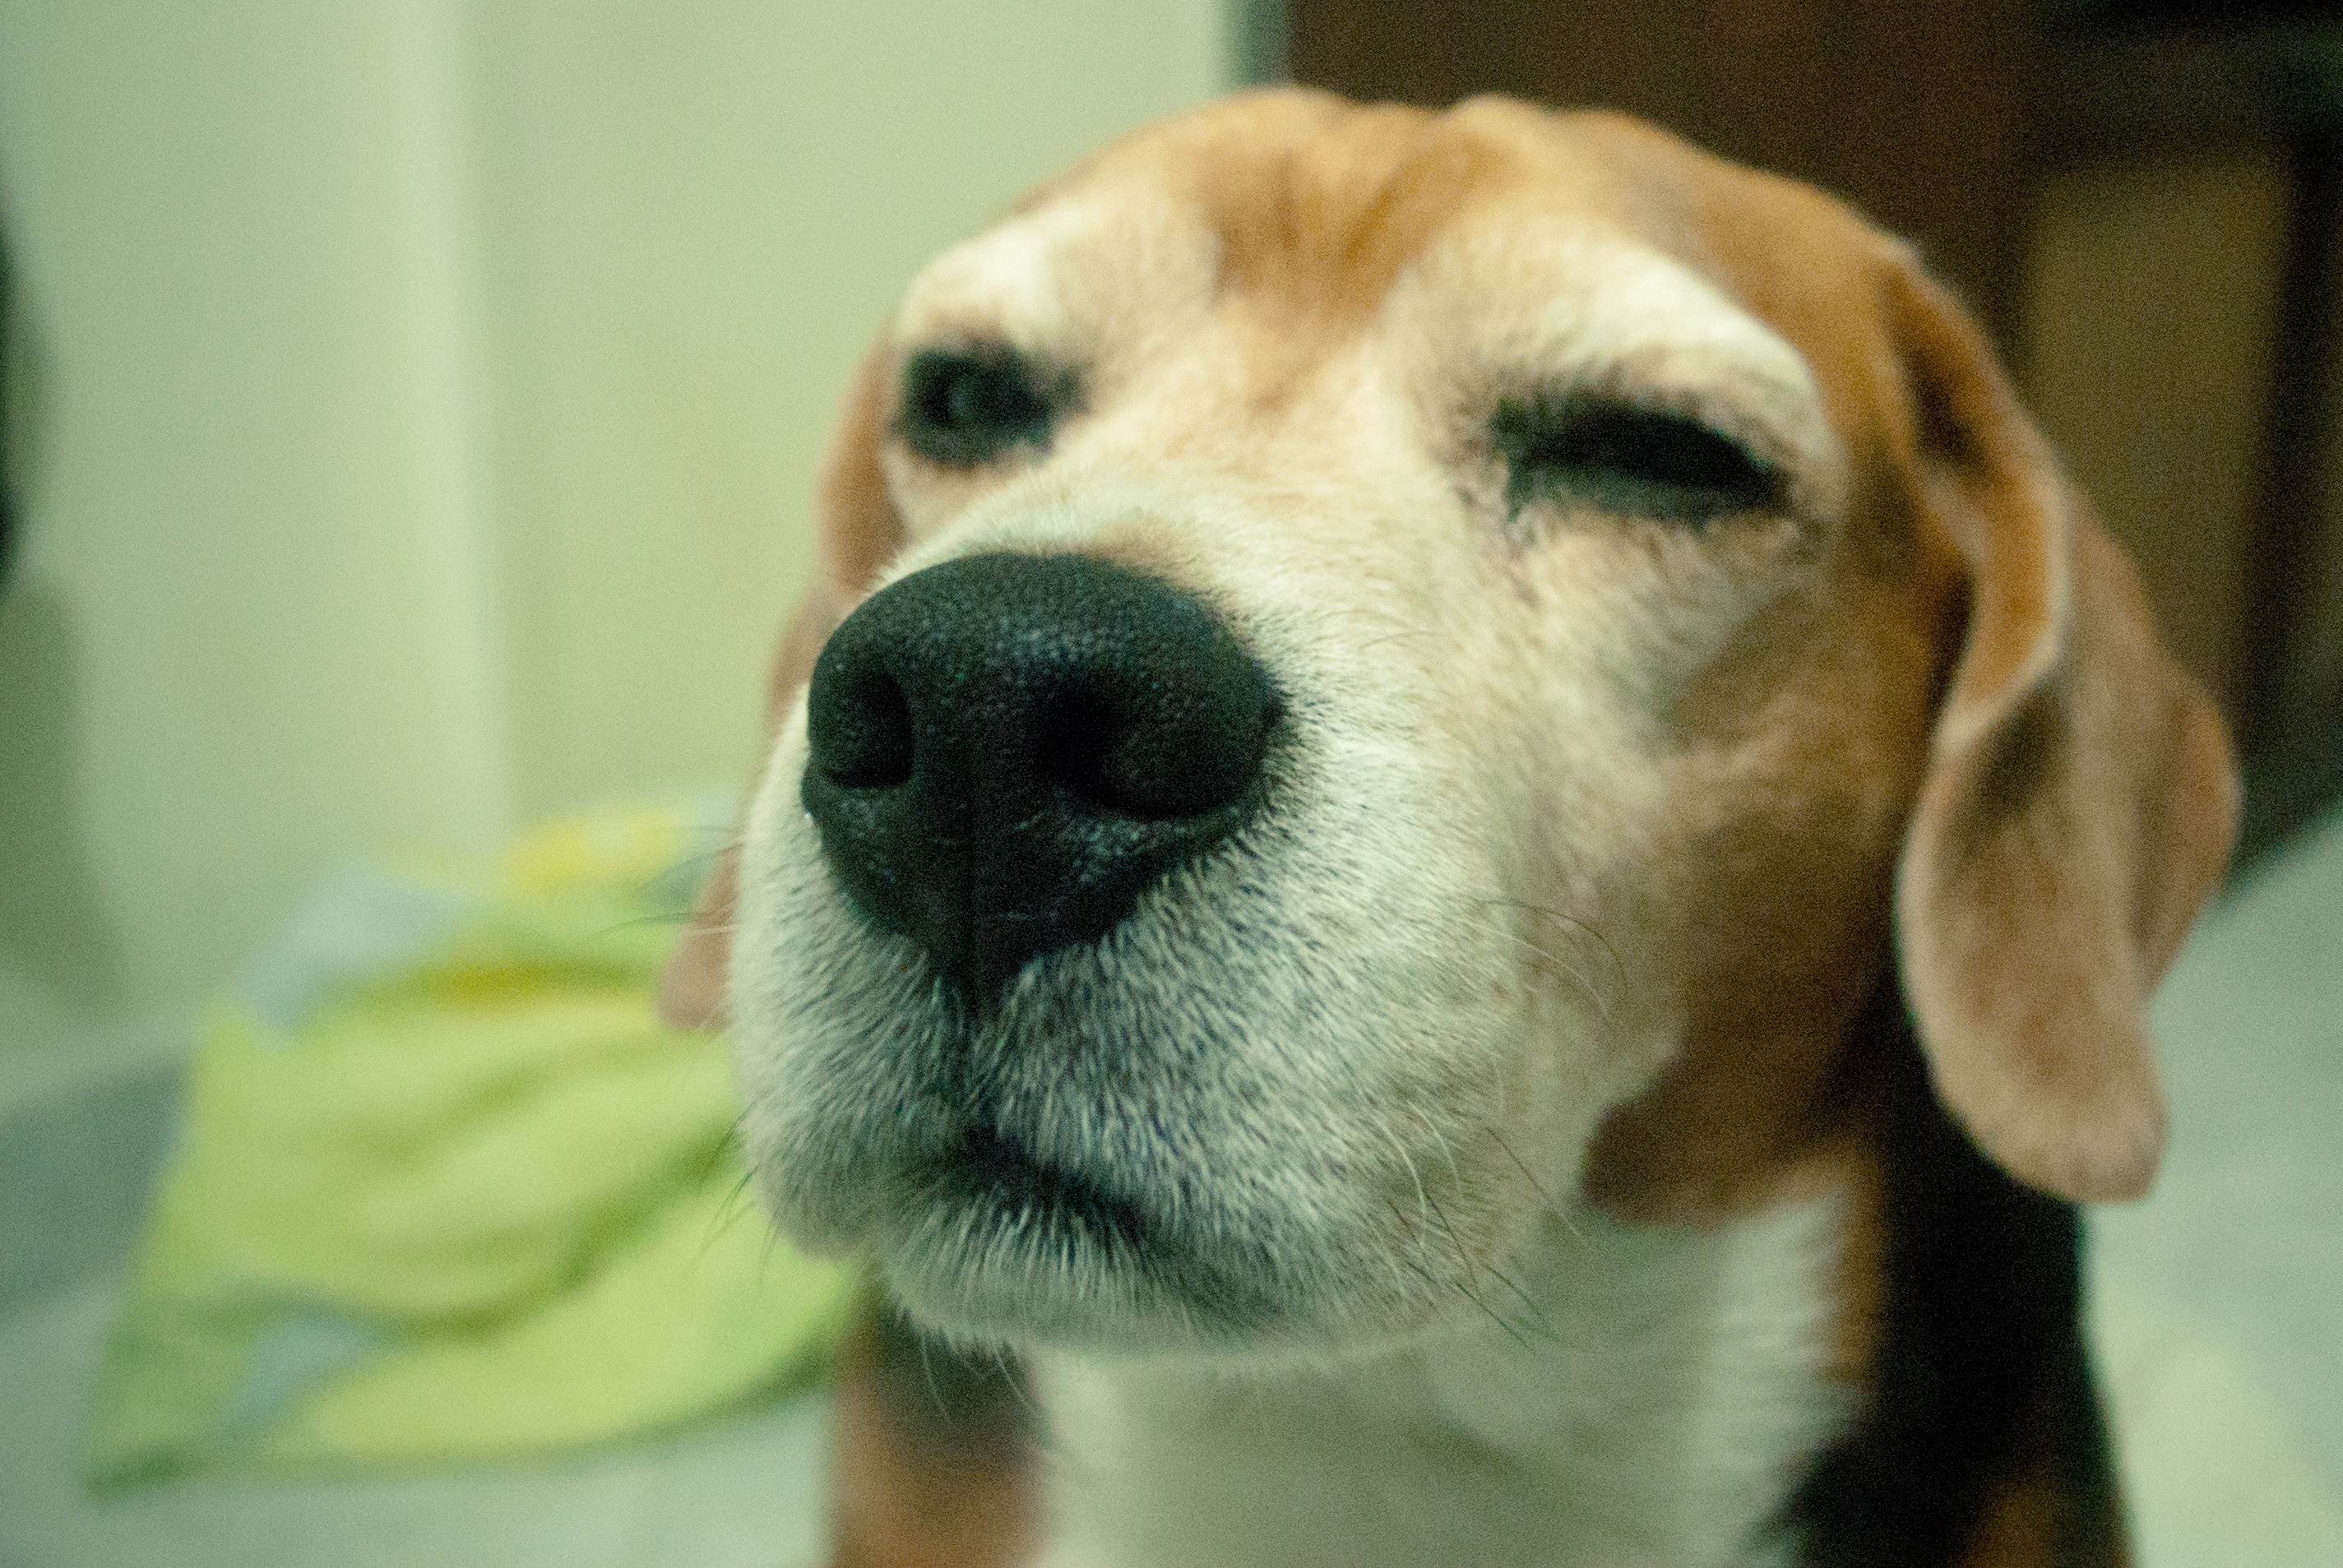
\includegraphics[width=0.2\textwidth]{image/suspicion.jpg}};
\end{tikzpicture}
\end{frame}

\begin{frame}[fragile]
\frametitle{Lossful Reasoning}
\framesubtitle{Sacrificing efficiency to gain unreliability}
So we write some tests:
\begin{lstlisting}[style=scala]
add10(0)        = 10
add10(5)        = 15
add10(-5)       = 5
add10(223)      = 233
add10(5096)     = 5106
add10(2914578)  = 29145588
add10(-2914578) = -29145568
\end{lstlisting}
And conclude, yes, this function adds ten to its argument
\end{frame}

\begin{frame}[fragile]
\frametitle{Lossful Reasoning}
\framesubtitle{Sacrificing efficiency to gain unreliability}
\begin{lstlisting}[style=scala]
def add10(n: Int): Int =
  if(n < 8000000) n + 10
  else n * 7
\end{lstlisting}
Wason Rule Discovery Test, \emph{confirmation bias\cite{gale2002does}}.
\end{frame}

\begin{frame}[fragile]
\frametitle{Lossful Reasoning}
\framesubtitle{Sacrificing efficiency to gain unreliability}
We will just write more tests!
\begin{lstlisting}[style=scala]
add10(18916712)  = 18916722
add10(-18916712) = -18916702
\end{lstlisting}
\ldots or we might come up with some system of apologetics for this shortfall
\begin{itemize}
  \item ``A negligent programmer has misnamed this function"
  \item ``More tests will fix it"
  \item ``Well we can't test everything!"
\end{itemize}
\end{frame}

\begin{frame}[fragile]
\frametitle{Lossful Reasoning}
\framesubtitle{Sacrificing efficiency to gain unreliability}
\begin{center}{We are reinforcing our excess confidence in our belief that we
are being responsible programmers}
\end{center}
\begin{center}{\textbf{We aren't}}
\end{center}
\end{frame}

\begin{frame}[fragile]
\frametitle{Lossful Reasoning}
\framesubtitle{Efficiency}
\begin{center}
Actually, we can do significantly better with a machine-checked proof,
mitigating our disposition to biases
\end{center}
\begin{center}{\emph{Automating "Automated Testing"?}}
\end{center}
\end{frame}

\begin{frame}[fragile]
\frametitle{Reasoning with parametricity}
\begin{block}{Monomorphic Signature}
\begin{itemize}
  \item Examining the signature \lstinline[style=scala]{Int => Int}
  \item We see a lot of things this function does \emph{not} do
  \item For example, it never returns \lstinline[style=scala]{"abc"}
  \item However, there is an unmanageable number of possible things it might do
\end{itemize}
\end{block}
\end{frame}

\begin{frame}[fragile]
\frametitle{Reasoning with parametricity}
\begin{block}{Another monomorphic example}
\begin{itemize}
  \item Examining the signature \lstinline[style=scala]{List[Int] => List[Int]}
  \item For example, it might add all the \lstinline{Int}s and return a list arrangement that depends on whether or not the result is a prime number
  \item The possibilities are \emph{enormous}
\end{itemize}
\end{block}
\end{frame}

\begin{frame}[fragile]
\frametitle{Reasoning with parametricity}
\begin{block}{Polymorphic Signature}
\begin{lstlisting}[style=scala]
def `irrelevant`[A](x: List[A]): List[A]
\end{lstlisting}
\begin{itemize}
  \item We can immediately assert, with confidence, a lot of things about how this function works \emph{because it is polymorphic}
  \item More directly, we assert what the function does not do
  \item<2> In other words, \emph{parametricity} has improved readability
  \item<2> Really? By how much?
\end{itemize}
\end{block}
\end{frame}

\begin{frame}[fragile]
\frametitle{Reasoning with parametricity}
\begin{lstlisting}[style=scala]
def `irrelevant`[A](x: List[A]): List[A] = 
  ...
\end{lstlisting}
\begin{theorem}Every element \lstinline{A} in the result list appears in the input. Contraposed, If \lstinline{A} is not in the input, it is not in the result\end{theorem}
\end{frame}

\begin{frame}[fragile]
\frametitle{Reasoning with parametricity}
\begin{block}{I know this because \ldots}
\begin{itemize}
  \item<1> Because I am the boss and I said so
  \item<2> Because Reliable Rob told me so
  \item<3> Because the \emph{function name} told me so
  \item<4> Because the comment told me so
  \item<5> \textbf{Because it would not have compiled otherwise}
\end{itemize}
\end{block}
\end{frame}

\begin{frame}[fragile]
\frametitle{Reasoning with parametricity}
\begin{block}{Uninhabited Example}
\begin{lstlisting}[style=scala]
def irrelevant[A, B](a: A): B = 
  ...
\end{lstlisting}
\end{block}
\begin{theorem}This function \textbf{never} returns because if it did, it would
never have compiled\end{theorem}
\end{frame}

\begin{frame}[fragile]
\frametitle{Reasoning with parametricity}
\begin{block}{Fast and loose reasoning is morally correct \cite{danielsson2006fast}}
\small{Functional programmers often reason about programs as if
they were written in a total language, expecting the results
to carry over to non-total (partial) languages. We justify
such reasoning.}
\end{block}
What does this mean exactly?
\end{frame}

\begin{frame}[fragile]
\frametitle{Fast and Loose Reasoning}
\begin{lstlisting}[style=scala]
def even(p: Int): Boolean = 
  ...
\end{lstlisting}
\begin{theorem}The \lstinline{even} function returns either \lstinline{true} or \lstinline{false}\end{theorem}
\end{frame}

\begin{frame}[fragile]
\frametitle{Fast and Loose Reasoning}
\begin{lstlisting}[style=scala]
def even(p: Int): Boolean = 
  even(p)
\end{lstlisting}
Actually, the \lstinline{even} function doesn't even return, \emph{yet we
casually exclude this possibility in discussion}.
\end{frame}

\begin{frame}[fragile]
\frametitle{Fast and Loose Reasoning}
\begin{block}{Scala has a \sout{few} lot of undermining escape hatches}
\begin{itemize}
  \item \lstinline{null}
  \item exceptions
  \item Type-casing (\lstinline{isInstanceOf})
  \item Type-casting (\lstinline{asInstanceOf})
  \item Side-effects
  \item \lstinline{equals}/\lstinline{toString}/\lstinline{hashCode}
  \item \lstinline{notify}/\lstinline{wait}
  \item \lstinline{classOf}/\lstinline{.getClass}
  \item General recursion
\end{itemize}
\end{block}
\end{frame}

\begin{frame}[fragile]
\frametitle{Fast and Loose Reasoning}
\framesubtitle{\lstinline{null} escape hatch}
\begin{lstlisting}[style=scala]
def `irrelevant`[A](x: List[A]): List[A] = 
  null
\end{lstlisting}
\begin{theorem}Every \lstinline{A} element in the result list appears in the input list\end{theorem}
Well, not if you don't even return a list.
\textbf{\lstinline$null$ breaks parametricity.}
\end{frame}

\begin{frame}[fragile]
\frametitle{Fast and Loose Reasoning}
\framesubtitle{\lstinline{type-casing} escape hatch}
\begin{lstlisting}[style=scala]
def `irrelevant`[A](x: A): Boolean = 
  x.isInstanceOf[Int] ||
  x match {
    case (s: String) => s.length < 10
  }
\end{lstlisting}
\begin{theorem}This function ignores its argument and consistently returns either \lstinline{true} or \lstinline{false}\end{theorem}
\textbf{Type-casing\footnote{case-analysis on type} breaks parametricity}
\end{frame}

\begin{frame}[fragile]
\frametitle{Fast and Loose Reasoning}
\framesubtitle{\lstinline{type-casting} escape hatch}
\begin{lstlisting}[style=scala]
def `irrelevant`[A](x: List[A]): List[A] = 
  "abc".asInstanceOf[A] :: x  
\end{lstlisting}
\begin{theorem}Every \lstinline{A} element in the result list appears in the input list\end{theorem}
\textbf{Type-casting breaks parametricity}
\end{frame}

\begin{frame}[fragile]
\frametitle{Fast and Loose Reasoning}
\framesubtitle{\lstinline{side-effect} escape hatch}
\begin{lstlisting}[style=scala]
def `irrelevant`[A](x: A): A = {
    println("hi")
    x
  }
\end{lstlisting}
\begin{theorem}This function only ever does one thing \textemdash return its argument \end{theorem}
\textbf{Side-effects breaks parametricity}
\end{frame}

\begin{frame}[fragile]
\frametitle{Fast and Loose Reasoning}
\framesubtitle{\lstinline{toString} escape hatch}
\begin{lstlisting}[style=scala]
def `irrelevant`[A](x: A): Int =
  x.toString.length
\end{lstlisting}
\begin{theorem}This function ignores its argument to return one of {${2^{32}}$} values. \end{theorem}
\textbf{Java's \lstinline$Object$ methods break parametricity}
\end{frame}

\begin{frame}[fragile]
\frametitle{Fast and Loose Reasoning}
\framesubtitle{where to place our trust?}
\begin{lstlisting}[style=scala]
def reverse[A, B](x: List[A]): List[B] = 
  x.foldLeft[List[B]](Nil)((b, a) =>
    a.`asInstanceOf`[B] :: b)
\end{lstlisting}
\begin{theorem}This function \textbf{always} returns \lstinline{Nil} and so cannot possibly reverse the list\end{theorem}
\textbf{Type-casting breaks parametricity}
\end{frame}

\begin{frame}[fragile]
\frametitle{Fast and Loose Reasoning}
\begin{itemize}
  \item Scala sure does have a lot of escape hatches!
  \item if we abandon all these escape hatches, to what extent is the programming environment disabled?
\end{itemize}
\end{frame}

\begin{frame}[fragile]
\frametitle{Fast and Loose Reasoning}
\begin{itemize}
  \item For example, Haskell disables side-effects, type-casing and type-casting, \emph{giving a significant advantage for no penalty}
  \item so what about Scala?
  \item can we use a reliable subset without too much penalty?
\end{itemize}
\end{frame}

\begin{frame}[fragile]
\frametitle{Fast and Loose Reasoning}
\frametitle{The Scalazzi Safe Scala Subset}
\begin{center}
Yes.
\end{center}
\begin{center}
And we do.
\end{center}
\end{frame}

\begin{frame}[fragile]
\frametitle{Fast and Loose Reasoning}
\begin{block}{The Scalazzi Safe Scala Subset}
\begin{itemize}
  \item \sout{\lstinline{null}}
  \item \sout{exceptions}
  \item \sout{Type-casing (\lstinline{isInstanceOf})}
  \item \sout{Type-casting (\lstinline{asInstanceOf})}
  \item \sout{Side-effects}
  \item \sout{\lstinline{equals}/\lstinline{toString}/\lstinline{hashCode}}
  \item \sout{\lstinline{notify}/\lstinline{wait}}
  \item \sout{\lstinline{classOf}/\lstinline{.getClass}}
  \item General recursion
\end{itemize}
\end{block}
\end{frame}

\begin{frame}[fragile]
\frametitle{Fast and Loose Reasoning}
\begin{block}{The Scalazzi Safe Scala Subset}
\begin{itemize}
  \item<1> We have now \textbf{improved} our reasoning abilities, but at what cost?
  \item<2> It turns out that eliminating these escape hatches results in a \textbf{significant language improvement} with minimal, orthogonal, easily-managed penalties
  \item<3> In other words, we can assume the language subset absent these attributes and by doing so, achieve a large net benefit
\end{itemize}
\end{block}
\end{frame}

\begin{frame}[fragile]
\frametitle{Fast and Loose Reasoning}
\framesubtitle{It works}
\begin{itemize}
  \item<1> Some open-source projects, using Scala, even Java and C\#, apply fast and loose reasoning to achieve confidence in the excellence of other team members
  \item<2> Project contributors rarely step on each others' (or their own) toes precisely because of this optimistic approach
  \item<3> Cynics fail hard
\end{itemize}
\end{frame}

\begin{frame}[fragile]
\frametitle{Fast and Loose Reasoning}
\framesubtitle{It works}
\begin{center}
Parametricity is principled and it works
\end{center}
\begin{center}
\includegraphics[height=3.8cm]{image/AbstractWigglyTwoppedHoopyWrapperZipdiddyQuip.png}
\end{center}
\begin{center}
Tell me again about this "real world." 
\end{center}
\end{frame}

\begin{frame}[fragile]
\frametitle{Scaling Parametricity}
\begin{lstlisting}[style=scala]
def forallM[F[_]: Monad, A]
  (p: A => F[Boolean], o: Option[A]): F[Boolean]
\end{lstlisting}
\begin{theorem}
  The \lstinline{Boolean} result depends on zero or more of
  \begin{itemize}
    \item None of its arguments
    \item Whether the \lstinline{Option} is a \lstinline{Some} or \lstinline{None}
    \item If the \lstinline{Option} is a \lstinline{Some}, then the result of having applied the given function to the \lstinline{Some} value
    \item \emph{Multiple applications of sequencing of the effect (\lstinline{F[Boolean]}) in the \lstinline{Some case}}
    \item in other words, one of \lstinline{(2 * 2 * 2)} inhabitants before accounting for multiple effect sequencing
  \end{itemize}
\end{theorem}
\end{frame}

\begin{frame}[fragile]
\frametitle{Scaling Parametricity}
  We conclude that, discounting multiple effect sequencing, there are 8 possible inhabitants \ref{forallM}:
  \begin{enumerate}
    \item always \lstinline{false}
    \item always \lstinline{true}
    \item \lstinline{o.isDefined}
    \item \lstinline{o.isEmpty}
    \item \lstinline{Some(a) => p(a) else false}
    \item \lstinline{Some(a) => p(a) else true}
    \item \lstinline{Some(a) => !p(a) else false}
    \item \lstinline{Some(a) => !p(a) else true}
  \end{enumerate}
\end{frame}

\begin{frame}[fragile]
\frametitle{Scaling Parametricity}
  \begin{block}{Importantly}
  The implementation may only use the monad primitive operations, even though the use-case may apply a specific monad context. If it were a specific monad (e.g. \lstinline{F=List}), the inhabitants become wildly unmanageable and the value of using the type for documentation hovers ever closer to zero.
  \end{block}
\end{frame}

\begin{frame}[fragile]
\frametitle{Scaling Parametricity}
  \begin{block}{For example}
  The \lstinline{forallM} function definitely does not perform any IO effects (\lstinline{F=IO}), even though the function user may apply that specific use-case
  \end{block}
  and so on \ldots
\end{frame}

\begin{frame}[fragile]
\frametitle{The Limits of Parametricity}
\begin{block}{monomorphic signature}
\begin{lstlisting}[style=haskell]
[Int] -> [Int]
\end{lstlisting}
From the \emph{\textbf{monomorphic} type}, what does this function do?
\end{block}

\includegraphics[width=0.2\textwidth]{image/shrug.png}
\end{frame}

\begin{frame}[fragile]
\frametitle{The Limits of Parametricity}
\begin{block}{theorems as types}
\begin{lstlisting}[style=csharp]
[a] -> [a]
\end{lstlisting}
From the \emph{\textbf{polymorphic} type}, what does this function do?
\end{block}
\large{\textbf{Theorem: all elements in the result appear in the input.}}

\tiny{How do we narrow down to disambiguity? How do we make up for this shortcoming?}
\end{frame}

\begin{frame}[fragile]
\frametitle{The Limits of Parametricity}
\begin{block}{theorems as types}
\begin{lstlisting}[style=csharp]
[a] -> [a]
\end{lstlisting}
\end{block}
We know a lot about what it does not do
\end{frame}

\begin{frame}[fragile]
\frametitle{The Limits of Parametricity}
\begin{block}{theorems as types}
\begin{lstlisting}[style=csharp]
[a] -> [a]
\end{lstlisting}
\end{block}
\emph{but we don't necessarily know exactly what it does do}
\end{frame}

\begin{frame}[fragile]
\frametitle{The Limits of Parametricity}
\begin{block}{We could}
\begin{itemize}
  \item<1-> write comments above the function

            \lstinline[style=csharp]{/* This function twiddles the database to twoddle out the twip twop */}

            \textbf{OR}
  \item<2-> write \emph{true} machine-checkable statements about the function
\end{itemize}
\end{block}
\end{frame}

\begin{frame}[fragile]
\frametitle{The Limits of Parametricity}
\begin{block}{what does this function do?}
\lstinputlisting[style=haskell]{source/reverse-with-tests.hs}
\end{block}
\end{frame}

\begin{frame}[fragile]
\frametitle{The Limits of Parametricity}
\begin{block}{what does this function do?}
\lstinputlisting[style=csharp,mathescape]{source/reverse-with-tests.cs}
\end{block}
\end{frame}

\begin{frame}[fragile]
\frametitle{The Limits of Parametricity}
\begin{block}{another example (Haskell)}
\begin{lstlisting}[style=haskell,mathescape]
flatMap :: (a -> List b) -> List a -> List b
flatMap = $\ldots$
\end{lstlisting}
\end{block}
\end{frame}

\begin{frame}[fragile]
\frametitle{The Limits of Parametricity}
\begin{block}{another example (C\#)}
\begin{lstlisting}[style=csharp,mathescape]
List<B> SelectMany<A, B>(this List<A>, Func<A, List<B>>) {
  $\ldots$
}
\end{lstlisting}
\end{block}
\end{frame}

\begin{frame}[fragile]
\frametitle{The Limits of Parametricity}
\begin{block}{another example}
\begin{lstlisting}[style=haskell,mathescape]
flatMap :: (a -> List b) -> List a -> List b
flatMap = $\ldots$
\end{lstlisting}
\begin{lstlisting}[style=csharp,mathescape]
List<B> SelectMany<A, B>(this List<A>, Func<A, List<B>>) {
  $\ldots$
}
\end{lstlisting}
\end{block}
\begin{itemize}
  \item If the input list is empty, so is the result
  \item Every \lstinline{(b)} in the result came from application of the given function
\end{itemize}
\end{frame}

\begin{frame}[fragile]
\frametitle{Once-inhabitance}
\begin{block}{sometimes tests are unnecessary}
\begin{lstlisting}[style=haskell]
f :: a -> a
\end{lstlisting}
\end{block}
\end{frame}

\begin{frame}[fragile]
\frametitle{Once-inhabitance}
\begin{block}{sometimes tests are unnecessary}
\begin{lstlisting}[style=haskell]
g :: Functor f => y -> f x -> f y
\end{lstlisting}
\end{block}
\emph{We already know that}
\begin{lstlisting}[style=haskell,mathescape]
$\lambda$> g "hi" [1,2,3]
["hi","hi","hi"]
\end{lstlisting}
\end{frame}

\begin{frame}[fragile]
\frametitle{Once-inhabitance}
\begin{block}{sometimes tests are \textbf{almost} unnecessary}
\begin{lstlisting}[style=haskell]
h :: a -> a -> a
\end{lstlisting}
\begin{lstlisting}[style=csharp]
A h<A>(A a1, A a2)
\end{lstlisting}
\end{block}
\end{frame}

\begin{frame}[fragile]
\frametitle{Once-inhabitance}
\begin{block}{sometimes tests are \textbf{almost} unnecessary}
\begin{lstlisting}[style=haskell]
h :: a -> a -> a
\end{lstlisting}
\begin{lstlisting}[style=csharp]
A h<A>(A a1, A a2)
\end{lstlisting}

\end{block}
\begin{lstlisting}[style=haskell,mathescape]
$\lambda$> h 7 8
7
\end{lstlisting}
\begin{lstlisting}[style=csharp]
csharp> h(7, 8)
7
\end{lstlisting}
\emph{We now know \textbf{precisely} what this function does}
\end{frame}

\begin{frame}[fragile]
\frametitle{Parametricity}
\begin{block}{non-trivial example}
\begin{lstlisting}[style=haskell]
both ::
  (Applicative f, Bitraversable r) =>
  (a -> f b) -> r a a -> f (r b b)
\end{lstlisting}
\end{block}
\begin{center}
What might this function do and what are the limitations of reasoning?
\end{center}
\end{frame}

\begin{frame}[fragile]
\frametitle{Parametricity}
\begin{block}{and so on}
\begin{lstlisting}[style=haskell]
point :: Store a b -> b

data Store a b = Store (a -> b) b
\end{lstlisting}
\end{block}
\end{frame}

\begin{frame}[fragile]
\frametitle{Parametricity}
\begin{block}{and on}
\begin{lstlisting}[style=haskell]
_1 :: Lens (a, x) (b, x) a b
\end{lstlisting}
\end{block}
\end{frame}

\input{conclusion}
\begin{frame}
\frametitle{References}

\bibliographystyle{amsalpha}
\bibliography{parametricity}

\end{frame}

\input{forallM}

\begin{frame}[fragile]
\frametitle{Workshop}
\begin{itemize}
\item Clone this git repository
      \lstinline$https://github.com/tonymorris/parametricity-exercises$
\item Install programming language environment:
      \begin{itemize}
      \item Haskell (\emph{recommended})
      \item Scala
      \item C\#
      \end{itemize}      
\end{itemize}
\end{frame}

\end{document}
